\section{The AWBS nonlocal transport model of electrons}
\label{sec:AWBSnonlocal}

In order to define a~nonlocal transport model of electrons, 
we use the~AWBS collision operator and the~P1 angular 
discretization of the~electron distribution function
\begin{equation}
  \tilde{\ft}(\vect{x}, \vn, \vmag) = 
  \fzero(\vect{x}, \vmag) + \vn\cdot\fone(\vect{x}, \vmag) , 
  \label{eq:P1approximation}
\end{equation}
consisting of the~isotropic part represented by the zeroth angular moment 
$\fzero = \frac{1}{4\pi}\int_{4\pi} \tilde{\ft} \dI\vn$ 
and the~directional part represented by the~first angular moment 
$\fone = \frac{3}{4\pi}\int_{4\pi} \vn
\tilde{\ft} \dI\vn$, where $\vn$ is the~transport direction (the~solid angle).
%It should be noticed, that \eqref{eq:P1approximation} represents 
%a~multi-dimensional equivalent to \eqref{eq:f_approximation}, where 
%the~following relations between the~spherical harmonics method
%and the~moments method hold $\ft^0 = \frac{\fzero}{4\pi}$ and 
%$\ft^1 = \frac{3}{4\pi}|\fone|$.
Then, the~first two angular moments
\cite{Shkarofsky_Particle_Kinetics_book_1966_24} applied to the~steady form of 
\eqref{eq:kinetic_equation} with collision operator \eqref{eq:AWBS_model} 
(extended by \eqref{eq:qAWBS_approximation}) lead to the~model equations
\begin{eqnarray}
  \vmag\frac{\nue}{2}\pdv{}{\vmag}\left(\fzero - \fM \right) &=&
  \frac{\vmag}{3}\nabla\cdot\fone + \frac{\qe}{\me}\frac{\E}{3}\cdot\left(
  \pdv{\fone}{\vmag} + \frac{2}{\vmag}\fone\right) , 
  \nonumber \\
  \label{eq:AP1f0}\\
  \vmag\frac{\nue}{2}\pdv{\fone}{\vmag}
  - \nuscat\fone &=& 
  \vmag\nabla\fzero + 
  \frac{\qe}{\me}\E\pdv{\fzero}{\vmag} 
  +\frac{\qe\B}{\me c}\vect{\times} \fone
  ,
  \nonumber \\
  \label{eq:AP1f1}
\end{eqnarray}
where $\nuscat = \nuei + \frac{\nue}{2}$. The system of equations 
\eqref{eq:AP1f0} and \eqref{eq:AP1f1} is called the~{\bf AP1 model} 
(AWBS + P1).  

On the~one hand side AP1 model gives us with the~information about 
the~electron distribution function, on the~other hand side 
a~macroscopic interpretation of the~microscopic EDF properties are of great
importance and provide the~bridge between kinetic and fluid description of 
plasma. For example the~\textit{flux} quantities as 
electric current and heat flux due to the~motion of electrons
\begin{equation}
  \vect{j} = \frac{4\pi}{3}\qe \int \vmag \fone~\dI\tilde{\vmag},~~ 
  \vect{q}_h = \frac{4\pi}{3}\frac{\me}{2} \int \vmag^3 \fone~\dI\tilde{\vmag},
  \nonumber
\end{equation}
where $\dI\tilde{\vmag} = \vmag^2\dI\vmag$ 
the~spherical coordinates metric,
are based on corresponding velocity moments (integrals) of the~first angular 
moment of EDF. Consequently, the~explicit formula for the~first angular moment
from \eqref{eq:AP1f1} (the~inversion inspired by \cite{Shkarofsky_1979_73})
proves to be extremely useful
\begin{equation}
  \fone = \frac{\nuscat^2 \vect{F}^* + \omegaB~\omegaB\cdot\vect{F}^* 
  - \nuscat~\omegaB \vect{\times} \vect{F}^*}{\nuscat (\omegaB^2 + \nuscat^2)}
  ,
  \label{eq:f1_explicit}
\end{equation} 
because it provides a~valuable 
information about the~dependence of macroscopic \textit{flux} quantities on
electric and magnetic fields in plasma, 
where $\omegaB = \frac{\qe\B}{\me c}$ is the~electron gyro-frequency and 
$\vect{F}^* = \vmag\frac{\nue}{2}\pdv{\fone}{\vmag} - \vmag\nabla\fzero 
 - \frac{\qe}{\me}\E\pdv{\fzero}{\vmag}$.

\subsection{Nonlocal Ohm's Law}
\label{sec:Efield}
The~expression \eqref{eq:f1_explicit} becomes extremely useful when used
to describe the~electron fluid momentum, i.e. the~current velocity moment
%\begin{equation}
%  \vect{j}(f, \vect{E}) = e \int \vmag \fone \vmag^2~\dI \vmag =
%  e \int \vmag \frac{\E^*}
%  {\nuei} \vmag^2~\dI \vmag ,
%  \label{eq:NonlocalOhm}
%\end{equation}
\begin{multline}
  \vect{j}_{(f, \E, \B)} = \qe \int \vmag \fone \vmag^2~\dI \vmag = \\
  - \frac{\qe^2}{\me} \int \vmag \frac{\nuei^2 \E^* 
  + \omegaB~\omegaB\cdot\E^* - \nuei~\omegaB \vect{\times} \E^*}
  {\nuei (\omegaB^2 + \nuei^2)}~\dI \tilde{\vmag} ,
  \nonumber %\label{eq:NonlocalOhm}
\end{multline}
where $\E^* = \E~\pdv{\fzero}{\vmag} + \frac{\me}{\qe}\vmag \nabla \fzero$ 
is the~effective electric field in plasma. 
This can be written as
\begin{equation}
  \vect{j}_{(f, \E, \B)} = \Iohm\pdv{\fzero}{\vmag}\E 
  + \frac{\me}{\qe} \Iohm\vmag \nabla \fzero
  ,
  \label{eq:NonlocalOhm}
\end{equation}
where we used the~following notation 
$\Iohm\vect{g} = - \frac{\qe^2}{\me} \int \vmag \frac{\nuei^2 \vect{g} 
  + \omegaB~\omegaB\cdot\vect{g} - \nuei~\omegaB \vect{\times} \vect{g}}
  {\nuei (\omegaB^2 + \nuei^2)}~\dI \tilde{\vmag}$ showing how $\Iohm$
acts on a~general vector field $\vect{g}$.
We refer to 
\eqref{eq:NonlocalOhm} as to the~{\bf nonlocal Ohm's law}.
Its relation and a~proper local asymptotic to the~standard Ohm's law  
can be found when $\fzero\rightarrow\fM$ and weak magnetization 
($\omegaB \ll \nuei$) is considered. Then \eqref{eq:NonlocalOhm} simplifies to
\begin{multline}
  \vect{j} =- \frac{\qe^2}{\me} \int \frac{\vmag^3}{\nuei}
  \left( \E~\pdv{\fM}{\vmag} + \frac{\me}{\qe}\vmag \nabla \fM \right)
  ~\dI \vmag =\\
  \frac{16\sqrt{\frac{2}{\pi}}\qe^2 \kB^\frac{3}{2} \Te^\frac{3}{2}}{\me^\frac{5}{2} \Gamma\Zbar}
  \left[\E - \frac{\frac{5}{2} \ed \kB \nabla \Te 
  + \nabla \ed \kB \Te}{\qe \ed}  \right] 
  ,
  \label{eq:AsymptoticOhm}
\end{multline}
which can be directly compared to the~local fluid theory 
%represented by the~\textit{generalized Ohm's law} 
\begin{equation}
  \E = \matr{\sigma}(\fzero)^{-1} \vect{j} 
  - \frac{\nabla P (\fzero)}{\qe \ed}
  \xrightarrow{\fzero \rightarrow \fM}
  \E_{l} = \frac{\vect{j}}{\sigma_{l}}
  + \frac{\nabla p_e - \vect{R}_{\Te}}{\qe \ed} 
  ,
  \label{eq:GeneralOhm} 
\end{equation}
while addressing properly the~local electric field $\E_{l}$ given by
the~pressure $p_e = \ed \kB \Te$,
the~thermal force $\vect{R}_{\Te} = - \frac{3}{2} \ed \kB \nabla \Te$ 
and the~local electrical conductivity 
$\sigma_{l} = 16\sqrt{\frac{2}{\pi}}\qe^2 \kB^\frac{3}{2} \Te^\frac{3}{2}
/ \me^\frac{5}{2} \Gamma\Zbar$ \cite{Braginskii_1965_3}.
In \eqref{eq:GeneralOhm} we defined the~nonlocal electrical tensor conductivity 
\begin{equation}
  \matr{\sigma} = \Iohm\pdv{\fzero}{\vmag}
  ,
  \label{eq:NonlocalSigma}
\end{equation}
and the~nonlocal microscopic force
\begin{equation}
  \nabla P = \matr{\sigma}^{-1}\me\ed \Iohm\vmag \nabla \fzero
  ,
  \label{eq:NonlocalGradP}
\end{equation}
based on \eqref{eq:NonlocalOhm}.

The~local dependence of the~AP1 current \eqref{eq:AsymptoticOhm} 
on electric field and gradients of $\ed$ and $\Te$ clearly demonstrates, 
that \eqref{eq:GeneralOhm} is a~local version of \eqref{eq:NonlocalOhm}.
This also implies that \eqref{eq:NonlocalOhm} provides a~very important 
physics related to the~magnetic field source in terms of nonlocal 
Biermann battery, since the~curl on the~electric field 
\eqref{eq:GeneralOhm} gives
\begin{equation}
  \nabla\vect{\times} \frac{\nabla P}{\qe \ed} 
  \xrightarrow{\fzero \rightarrow \fM} 
  \nabla\vect{\times} \frac{\nabla p_e - \vect{R}_{\Te}}{\qe \ed} =
  \frac{\kB}{\qe\ed}\nabla \Te \vect{\times}\nabla \ed
  .
  \label{eq:NonlocalBiermann}
\end{equation}

A~local version of the~{\bf nonlocal Ohm's law} \eqref{eq:NonlocalOhm} 
compared to the~\textit{generalized Ohm's law} \eqref{eq:GeneralOhm} when
a~magnetic field is applied would require a~much more delicate analysis and 
we leave it as a~future complementary work.

It should be noted, that $\nue$-related terms in \eqref{eq:f1_explicit} 
have been omitted in \eqref{eq:NonlocalOhm}, 
since the~e-e collisions do not contribute 
(cancel out when integrated over velocity) to the~momentum
change, i.e. 
$\int \vmag \left( \vmag\frac{\nue}{2}\pdv{\fone}{\vmag}
  - \frac{\nue}{2}\fone\right) \dI\tilde{\vmag} = 0$.

\begin{comment} % Ohm's law with B.
\begin{eqnarray} 
  \E &=&  
  \frac{\nabla p_e - \vect{R}_{\Te}}{\qe \ed}
  +~~~~~~~~ 
  \frac{\vect{j}}{\sigma} 
  ~~~~~~-~~~~~~ 
  \frac{\vect{j}\vect{\times}\B}{\qe\ed c} 
  ,
  \nonumber \\
  %\E 
  %&=& 
  %\frac{\int \vmag^2 \nabla \fzero \vmag^2\, \dI \vmag}
  %{\int \vmag \pdv{\fzero}{\vmag} \vmag^2\, \dI \vmag}
  %+  
  %\frac{\int \vmag \nuei\fone \vmag^2\, \dI \vmag}
  %{\int \vmag \pdv{\fzero}{\vmag} \vmag^2\, \dI \vmag} 
  %+ 
  %\frac{\int \vmag \fone\times\B \vmag^2\, \dI \vmag}
  %{\int \vmag \pdv{\fzero}{\vmag} \vmag^2\, \dI \vmag} 
  %.
  %\nonumber
  \frac{\qe}{\me}\E 
  &=& 
  \frac{\int \vmag^2 \nabla \fzero~\dI \tilde{\vmag}}
  {\int \vmag \pdv{\fzero}{\vmag}~\dI \tilde{\vmag}}
  +  
  \frac{\int \vmag \nuei\fone~\dI \tilde{\vmag}}
  {\int \vmag \pdv{\fzero}{\vmag}~\dI \tilde{\vmag}} 
  + 
  \frac{\qe\int \vmag \fone\vect{\times}\B~\dI \tilde{\vmag}}
  {\me c \int \vmag \pdv{\fzero}{\vmag}~\dI \tilde{\vmag}} 
  .
  \nonumber
\end{eqnarray}
\end{comment} % Ohm's law with B.

\subsection{AWBS Nonlocal Magneto-Hydrodynamics}
\label{sec:ANTH}
The~\textit{AWBS nonlocal~magneto-hydrodynamic~model} (Nonlocal-MHD)
refers to two~temperature single-fluid hydrodynamic model 
extended by a~kinetic model of electrons using the~AWBS transport equation,
which provides a~direct coupling between hydrodynamics and Maxwell equations.

Mass, momentum density, and total energy 
$\rho$, $\rho\vect{u}$, and 
$E = \frac{1}{2}\rho\vect{u}\cdot\vect{u} + 
 \rho \varepsilon_i + \rho \varepsilon_e$, 
where $\rho$ is 
the~density of plasma, $\vect{u}$ the~plasma fluid velocity, $\varepsilon_i$ 
the~specific internal ion energy density, 
and $\varepsilon_e$ the~specific internal 
electron energy density,
are modeled by the~Euler equations in Lagrangian frame 
\cite{Holec_DGBGKT_2016, Holec_PoPNTH2018}
\begin{eqnarray}
 \frac{\dI \rho}{\dI t} &=& - \rho\nabla\cdot\vect{u}
 , 
 \label{eq:NTH_rho}\\
 \rho\, \frac{\dI \vect{u}}{\dI t} &=& - \nabla (p_i + p_e) 
 + \vect{j}_{(f, \E, \B)} \vect{\times}\B
 ,  
 \label{eq:NTH_v}\\
 \rho~C_{V_i}\frac{\dI \Ti}{\dI t} 
 &=& 
 \left(\rho^2 C_{\Ti} - p_i\right)\nabla\cdot\vect{u} 
 - G(\Ti - \Te)
 ,  
 \label{eq:NTH_Ti}\\
 \rho~C_{V_e} \frac{\dI \Te}{\dI t}
  %+ \frac{\dI \epsilon_R}{\dI t} 
  &=& 
 \left(\rho^2 C_{\Te} - p_e \right) \nabla\cdot\vect{u}  
 + G(T_i - \Te)
 \nonumber\\ 
 && - \nabla\cdot\vect{q}_{h(f, \E, \B)} + Q_{\text{IB}} 
 , 
 \label{eq:NTH_Te}
\end{eqnarray}
where $\Ti$ is the~temperature of ions, $\Te$ the~temperature of electrons,
$p_i$ the~ion pressure, $p_e$ the~electron pressure,
$\vect{q}_h$ the~heat flux, $Q_{\text{IB}}$ the~inverse-bremsstrahlung laser 
absorption, and 
$G = \rho C_{V_e} \nuei$ is 
the~ion-electron energy exchange rate. 
The~thermodynamic closure terms 
$p_e$, $p_i$, 
$C_{V_i} = \frac{\partial \varepsilon_i}{\partial \Ti}$, 
$C_{\Ti} = \pdv{\varepsilon_i}{\rho}$,
$C_{V_e} = \frac{\partial \varepsilon_e}{\partial \Te}$, 
$C_{\Te} = \pdv{\varepsilon_e}{\rho}$
%$\frac{\partial \varepsilon_e}{\partial T_e}$,
%$\frac{\partial \varepsilon_i}{\partial T_i}$,
%$\frac{\partial \varepsilon_e}{\partial \rho}$,
%$\frac{\partial \varepsilon_i}{\partial \rho}$ 
are obtained from an~equation of state (EOS), e.g.
the~SESAME equation of state tables
\cite{T4_SESAME_83, Lyon_SESAME_EOS_database-TechRep-92}.

The~magnetic and electric fields are modeled by Maxwell equations
\begin{eqnarray}
  \frac{1}{c}\frac{\dI \B}{\dI t} &=& - \nabla\vect{\times}\E
  ,
  \label{eq:Faraday} \\
  \frac{1}{c}\frac{\dI \E}{\dI t} &=& \nabla\vect{\times}\B - \frac{4\pi}{c}
  \vect{j}_{(f, \E, \B)}
  ,
  \label{eq:Ampere}
  %\frac{4\pi}{c}
  %\vect{j}(f, \vect{E}) &=& \nabla\vect{\times}\vect{B} ,
\end{eqnarray}
where the~initial state of $\B$ and $\E$ obeys the~Gauss's law.

We have explicitly written the~current and heat flux as dependent on
electron kinetics, represented by the~electron distribution function $f$,
and electric and magnetic fields. In principal, $\vect{j}_{(f, \E, \B)}$
and $\vect{q}_{h(f, \E, \B)}$ can be referred to as the~\textit{kinetic closure}
and is provided by the~{\bf AP1 model} \eqref{eq:AP1f0} and \eqref{eq:AP1f1},
where $\fM$ is given on the~spatial profile of $\Te$ 
governed by \eqref{eq:NTH_Te}.
All quantities are defined in the~fluid frame in the aforementioned 
Nonlocal-MHD model.
%especially that 
%$\nabla\vect{\times} \nabla \fzero \sim \nabla\vect{\times} \nabla p_e \sim \nabla \ed \vect{\times} \nabla \Te$

\subsection{Numerical Implementation of the AWBS Electron Kinetics}
\label{sec:Numerics}

It is well known, that as the~electron transport exhibits a~quasi-steady
behavior, the~same holds for the~electric field in \eqref{eq:Ampere} on 
the~time scale of the~fluid. Consequently, the~Ampere's law \eqref{eq:Ampere} 
usually takes a~quasi-steady form 
$\frac{4\pi}{c} \vect{j}_{(f, \E, \B)} = \nabla\vect{\times}\B$
when used in hydrodynamics. Proceeding further, one can make use of 
the~{\bf nonlocal Ohm's law} \eqref{eq:NonlocalOhm} to write 
a~\textit{fully kinetic form of the~Ampere's law} 
governing the~electric field $\E$
\begin{equation}
  \Iohm\pdv{\fzero}{\vmag}\E 
  + \frac{\me}{\qe} \Iohm\vmag \nabla \fzero = 
  \frac{c}{4\pi} \nabla\vect{\times}\B 
  .
  \label{eq:AmpereKinetic}
\end{equation}

In order to solve the~kinetics of electrons, we adopt a~high-order 
finite element discretization 
\cite{Dobrev_Kolev_Rieben-High-order_curvilinear_finite_element_methods_for_Lagrangian_hydrodynamics, mfem-library} 
of the~model equations \eqref{eq:AP1f0}, \eqref{eq:AP1f1}, 
\eqref{eq:AmpereKinetic}
\begin{eqnarray}
  \matr{M}^{L_2}_{_{(\frac{\vmag\nue}{2})}}\cdot\ddv{\vfzero}{\vmag} 
  - \matr{V}^{L_2}_{_{(\frac{\qe\E}{3\me})}}\cdot\ddv{\fone}{\vmag}
  &=&
  \matr{D}^{L_2}_{_{(\frac{\vmag}{3})}}\cdot\fone 
  + \matr{M}^{L_2}_{_{(\frac{2\qe\E}{3\me\vmag})}}\cdot\fone
  \nonumber \\ 
  &&+ \vect{b}^{L_2}_{_{(\frac{\vmag\nue}{2}\pdv{\fM}{\vmag})}}, 
  \label{eq:FEMAP1f0}
  \\
  \matr{M}^{H_1}_{_{(\frac{\vmag\nue}{2})}}\cdot\ddv{\fone}{\vmag}
  - \matr{V}^{H_1}_{_{(\frac{\qe\E}{\me})}}\cdot\ddv{\vfzero}{\vmag}
   &=& 
  \matr{G}^{H_1}_{_{(\vmag)}}\cdot\vfzero 
  + \matr{M}^{H_1}_{_{(\nuscat)}}\cdot\fone 
  \nonumber \\
  && + \matr{C}^{H_1}_{_{(\frac{\qe\B}{\me c}\vect{\times})}}\cdot\fone
  ,
  \label{eq:FEMAP1f1}\\
  \matr{J}^{ND}_{_{(\pdv{\fzero}{\vmag})}}\cdot\E 
  &=& 
  \matr{JG}^{ND}_{_{(\frac{\me\vmag}{\qe})}}\cdot\vfzero
  + \vect{b}^{ND}_{_{(\frac{c}{4\pi} \nabla\vect{\times}\B)}} 
  ,
  \nonumber \\
  \label{eq:FEMAmpereKinetic}
\end{eqnarray}
where the~continuous differential operators are represented by standard 
discrete analogs (matrices of bilinear forms) 
$\matr{M}, \matr{G}, \matr{D}, \matr{V}, \matr{C}$, i.e. mass, gradient, 
divergence, vector field dot product, and vector field curl, and
by $\matr{J}, \matr{JG}$ matrices specific to {\bf nonlocal Ohm's law} 
\eqref{eq:NonlocalOhm}. The~linear form $\vect{b}$ represents sources, i.e.
temperature $\Te$ via $\pdv{\fM}{\vmag}$ and the~curl of 
the~magnetic field $\B$. These finite element discrete analogs are defined
on piece-wise continuous $L_2$ finite element space (domain of $\vfzero$),
continuous $H_1$ finite element space (domain of $\fone$) 
\cite{Dobrev_Kolev_Rieben-High-order_curvilinear_finite_element_methods_for_Lagrangian_hydrodynamics}, 
and Nedelec finite element space (domain of $\E$). We do not show their
definitions since it is out of the~scope of this article. 

The~strategy of solving 
\eqref{eq:FEMAP1f0} and \eqref{eq:FEMAP1f1} resides in integrating 
$\ddv{\vfzero}{\vmag}$
and $\ddv{\fone}{\vmag}$ along the~velocity magnitude. 
This is done by starting the~integration
from infinite velocity ($\vmag = 7 \vth^{max}$ is a~sufficiently high limit) 
to zero velocity using the~Implicit Runge-Kutta method. The~value
$\vth^{max}$ equals the~electron thermal velocity corresponding to the~maximum 
electron temperature in the~current profile of plasma.
It should be noted, that the~backward integration concept is crucial for 
the~model, since it corresponds to the~deceleration of electrons due to 
collisions \cite{Touati_2014}, which leads to some limitations described in 
\appref{app:AP1limit}. 



\section{Benchmarking the~AWBS nonlocal transport model}
\label{sec:BenchmarkingAWBS}
After having shown several encouraging properties of the~AWBS transport 
equation defined by \eqref{eq:AWBS_model} under local diffusive conditions
in \secref{sec:DiffusiveKinetics}, this section provides a~broader analysis
of the~electron transport and focuses on analysis its behavior under variety of
conditions in plasmas. In principle, this is characterized by allowing that
electron mean free path can be arbitrarily long, which leads to so-called 
nonlocal electron transport extensively investigated in numerous publications 
\cite{Malone_1975_15, Colombant_PoP2005, Bell_1981_83, LMV_1983_7, Brantov_Nonlocal_electron_transport_1998, schurtz2000, Sorbo_2015}.
Among a~variety of tests suitable for benchmarking the~nonlocal electron 
transport models published 
\cite{Epperlein_PoFB1991, marocchino2013, Sorbo_2015, 
Sorbo_2016, Sherlock_PoP2017, Brodrick_PoP2017}, we focus on 
conditions relevant to inertial confinement fusion plasmas generated by lasers.
%Since the~Fokker-Planck modeling of electrons in ICF 
%plasma \eqref{eq:LFP_model} represents an~essential tool. Being so, 

We introduce our implementation of the~AWBS nonlocal transport model presented
in \secref{sec:AWBSnonlocal} called AP1,
where its results are further benchmarked against simulation results
provided by Calder, a~collisional Particle-In-Cell
code, and by Aladin and Impact VFP codes. 
Their description follows in the~next section.

%\begin{figure}[tbh]
%  \begin{center}
%    \begin{tabular}{c}
%      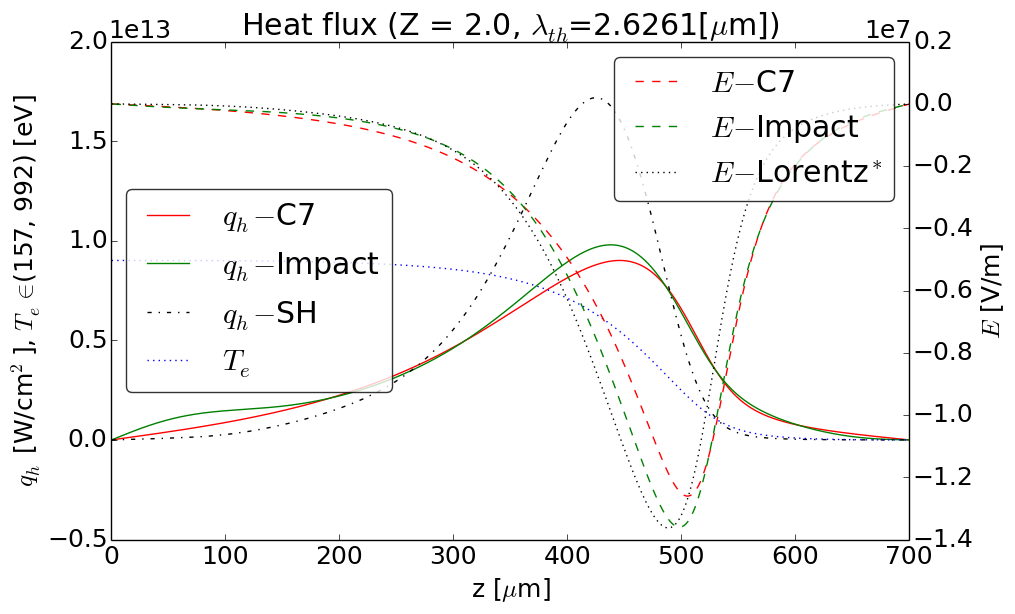
\includegraphics[width=\figscale\textwidth]{../VFPdata/C7_Impact_case3_heatflux.png} \\
%      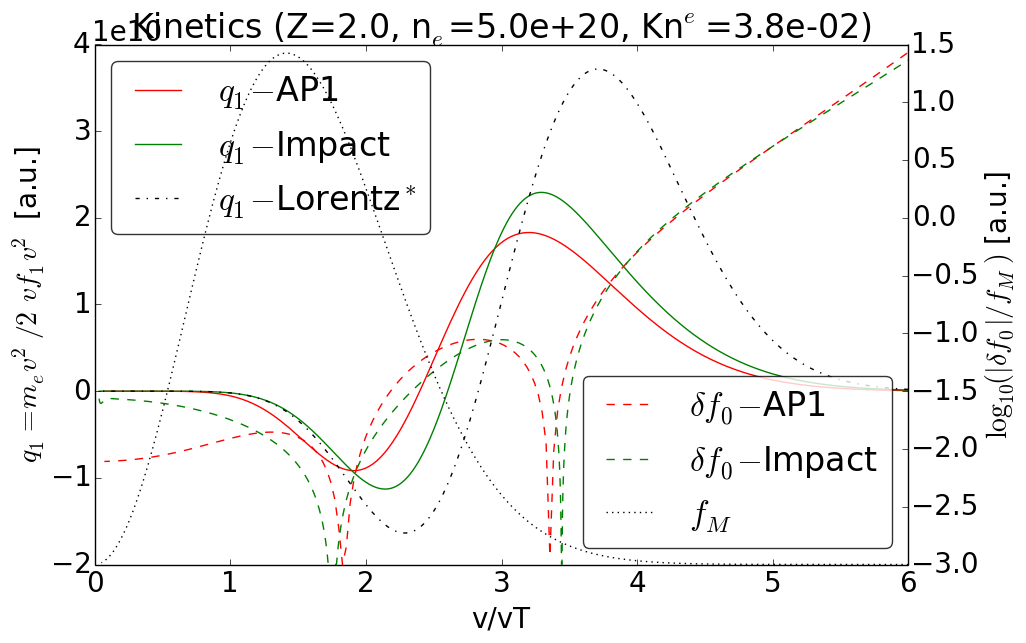
\includegraphics[width=\figscale\textwidth]{../VFPdata/C7_Impact_case3_kinetics.png}
%    \end{tabular}
%  \caption{  
%  Snapshot 12 ps. Left: correct steady solution of heat flux. 
%  Right: correct comparison to kinetic profiles at point 437 $\mu$m by Impact.
%  Velocity limit 4.0 $\vth$.
%  }
%  \label{fig:C7_Impact_case3}
%  \end{center} 
%\end{figure}

%\subsection{Aladin, Impact, and Calder kinetic codes}
%\label{sec:AladinImpactCaldercodes}

%%% CEA contribution starts
\textbf{Calder PIC code}

In the~limit of classical physics, a~fluid description of the~particle 
phase-space, including small angle binary collisions, can be described with 
the~Maxwell equations \eqref{eq:Faraday}, \eqref{eq:Ampere}
%\begin{eqnarray}
%&&\nabla\cdot \mathbf{E}=\sum_\alpha \frac{q_\alpha}{\varepsilon_0} n_{\alpha},\\
%&&\nabla\cdot \mathbf{B}=0,\\
%&&\nabla\vect{\times} \mathbf{E}+\frac{\partial \mathbf{B}}{\partial t}=0,\\
%&&\nabla\vect{\times} \mathbf{B}-\mu_0\varepsilon_0\frac{\partial \mathbf{E}}{\partial t}=\mu_0\sum_\alpha\mathbf{j}_{\alpha},\label{maxw}
%\end{eqnarray}
coupled with the~ion and electron Vlasov equations with 
the~Landau-Beliaev-Budker collisions integral (LBB)
\cite{Landau_1936, Beliaev_SPD1956} 
\begin{multline}
\frac{\partial f_\alpha}{\partial t}+\mathbf{v}\cdot\nabla_{\mathbf{x}}f_\alpha+q_\alpha\left(\mathbf{E}+\mathbf{v}\vect{\times}\mathbf{B}\right)\nabla_{\mathbf{p}}f_\alpha =
\\
C_{LBB}(f_\alpha,f_\alpha)+\sum_\beta C_{LBB}(f_\alpha,f_\beta)
.
\end{multline}
The LBB collision integral takes the~form
\begin{multline}
C_{LBB}(f_\alpha,f_\beta)=
\\
-\frac{\partial}{\partial \mathbf{p}}\cdot\frac{\Gamma_{\alpha\beta}}{2}\left[\int \mathbf{U}(\mathbf{p},\mathbf{p}^\prime)\cdot(f_\alpha\nabla_{\mathbf{p}^\prime}f_\beta^\prime-f_\beta^\prime\nabla_{\mathbf{p}}f_\alpha)\right]d^3\mathbf{p}^\prime
,
\label{eq:LBB_model}
\end{multline}
where its relativistic kernel reads
$\mathbf{U}(\mathbf{p},\mathbf{p}^\prime)=\frac{r^2/\gamma\gamma^\prime}{(r^2-1)^{3/2}}$ 
$\left[(r^2-1)\mathbf{I}-\mathbf{p}\otimes\mathbf{p}-\mathbf{p}^\prime\otimes\mathbf{p}^\prime+r(\mathbf{p}\otimes\mathbf{p}^\prime+\mathbf{p}^\prime\otimes\mathbf{p})\right]$
with $\gamma=\sqrt{1+\mathbf{p}^2}$, $\gamma^\prime=\sqrt{1+\mathbf{p}^{\prime 2}}$ and $r=\gamma\gamma^\prime-\mathbf{p}\cdot\mathbf{p}^\prime$. 
The momemtum $\mathbf{p}_\alpha$ ($\mathbf{p}_\beta$) is normalized to 
$m_\alpha c$ (resp. $m_\beta c$). The~collision operator \eqref{eq:LBB_model} 
tends to \eqref{eq:LFP_model} in the non-relativistic limit.
%described in Appendix~\ref{app:CalderKinetics}. 
%The~latter is the~relativistic version of the~collision operator 
%introduced in \eqref{eq:LFP_model}. 
The aforementioned model is solved in 3D by the PIC code CALDER. 
\cite{Lefebvre_NF2003, Perez_PoP2012}.
Brief description of the Calder code \figref{fig:C7_Calder_case1}.

\textbf{Impact and Aladin VFP codes}

The~PIC code is extremely expensive as the~collisions require the~description 
of the~velocity space in 3 dimensions. Yet, a~reduction of dimensions can be 
done by developing the~distribution function in a~cartesian tensor series, 
equivalent to a~serie along the spherical harmonics \cite{Johnston_PR1960}
as follows:
\begin{equation}
  f(t,\mathbf{x},\vv) = f_0(t,\mathbf{x},\vmag) 
  + \vn\cdot \vect{f}_1(t,\mathbf{x},\vmag)
  +\vn\otimes\vn:\matr{f}_2(t,\mathbf{x},\vmag)+... .
  \label{Pn}
\end{equation}
%where $v=|\mathbf{v}|$, $\Omega=\mathbf{v}/v$. 
A P$_n$ model refers to 
neglecting orders higher than $\matr{f}_n$. The distribution function 
approximation $f(t,\mathbf{x},\vv)\approx f_0(t,\mathbf{x},\vmag)
+\vn\cdot \vect{f}_1(t,\mathbf{x},\vmag)$ coupled with 
the~Landau-Fokker-Planck collisional operator 
\eqref{eq:LFP_model}, leads to the P$_1$-VFP model 
\cite{Johnston_PR1960, Kingham_JCP2004}:
\begin{eqnarray}
\frac{\partial f_0}{\partial t}+\frac{\vmag}{3}\nabla \cdot f_1
+\frac{\qe}{3\me\vmag^2}\frac{\partial}{\partial \vmag}(\vmag^2\E\cdot \mathbf{f}_1)
&=&
C^0_{ee}(f_0) ,
 \label{eq:P1f0_Aladin}\\
\frac{\partial \mathbf{f}_1}{\partial t}+\vmag\nabla f_0
+ \frac{\qe\E}{\me}\frac{\partial f_0}{\partial \vmag}
+\frac{\qe\B}{\me}\vect{\times} \mathbf{f}_1 
&=&
- \nuei\mathbf{f}_1 .
\label{eq:P1f1_Aladin}
\end{eqnarray}
where for simplicity only the~isotropic 
contribution of \eqref{eq:LFP_model} is used 
\begin{eqnarray} 
C^0_{ee}(f_0) &=& \frac{\Gamma}{v^2}\frac{\partial}{\partial \vmag}
\left[C(f_0)f_0+D(f_0)\frac{\partial f_0}{\partial \vmag}\right] ,
\\
C(f_0(\vmag)) &=& 4\pi\int_0^\vmag f_0(u) u^2 \dI u ,
\\
D(f_0(\vmag)) &=& \frac{4\pi}{\vmag}\int_0^\vmag u^2\int_u^\infty w f_0(w) 
\dI w \dI u .
\end{eqnarray}

\begin{comment} % Hydro quantities.
The electron and energy densities are obtained from the isotropic part of the distribution function $f_0$:
\begin{eqnarray}
n_e=4\pi\int_{\mathbf{R}^+} f_0v^2dv,\\
U_e=2\pi m_e\int_{\mathbf{R}^+} f_0v^4dv,
\end{eqnarray}
and the electron current and heat flux are obtained from the anisotropic part of the distribution function $\mathbf{f}_1$:
\begin{eqnarray}
\mathbf{j}_e=-\frac{4\pi e}{3}\int_{\mathbf{R}^+} \mathbf{f}_1v^3dv,\\
\mathbf{Q}_e=\frac{2\pi m_e}{3}\int_{\mathbf{R}^+} \mathbf{f}_1v^5dv.
\end{eqnarray}
\end{comment} % Hydro quantities.

Impact and Aladin solve the system \eqref{eq:P1f0_Aladin} 
and \eqref{eq:P1f1_Aladin} with the Maxwell equations  
\eqref{eq:Faraday} and \eqref{eq:Ampere} in two dimensions, 
assuming motionless ions.
Brief description of the Aladin code \figref{fig:C7_Aladin_case5}, \figref{fig:C7_Aladin_case3}.


%%% CEA contribution ends

%\begin{itemize}
%  \item Brief description of the Impact code \figref{fig:C7_Impact_case3}.
%\end{itemize}

\begin{figure}[tbh]
  \begin{center}
    \begin{tabular}{c}
      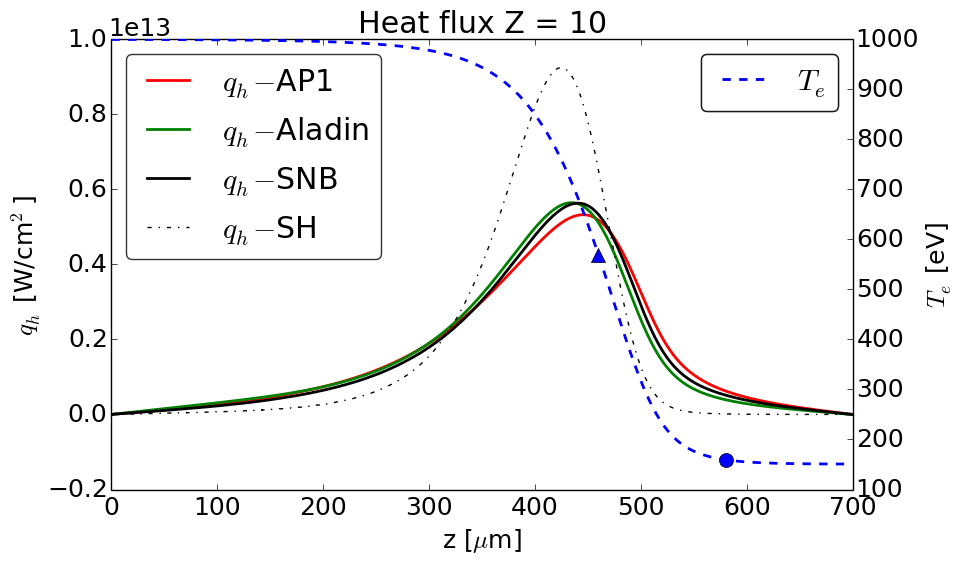
\includegraphics[width=\figscale\textwidth]{../VFPdata/C7_Aladin_case3_heatflux.png} \\
      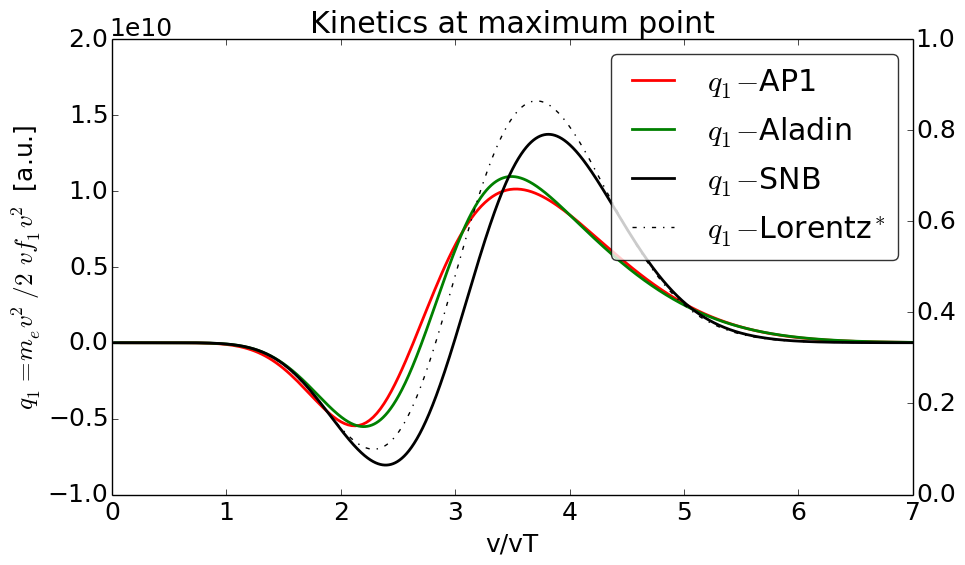
\includegraphics[width=\figscale\textwidth]{../VFPdata/C7_Aladin_case3_kinetics.png} \\
      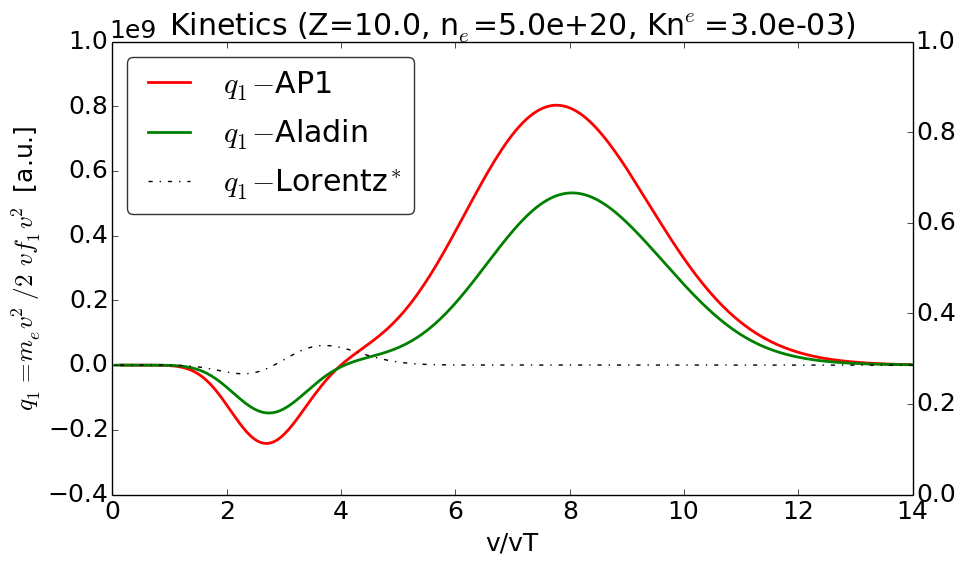
\includegraphics[width=\figscale\textwidth]{../VFPdata/C7_Aladin_case3_nonlocal_kinetics.png}  
    \end{tabular}
  \caption{  
  Snapshot 12 ps. Top: correct steady solution of heat flux.  
  Middle: correct comparison to kinetic profiles at point 442 $\mu$m by Aladin. 
  Velocity limit 3.4 $\vth$.
  Bottom: correct comparison to kinetic profiles at point 550 $\mu$m by Aladin.
  Velocity limit 8.8 $\vth$
  }
  \label{fig:C7_Aladin_case3}
  \end{center} 
\end{figure}

\begin{figure}[tbh]
  \begin{center}
    \begin{tabular}{c}
      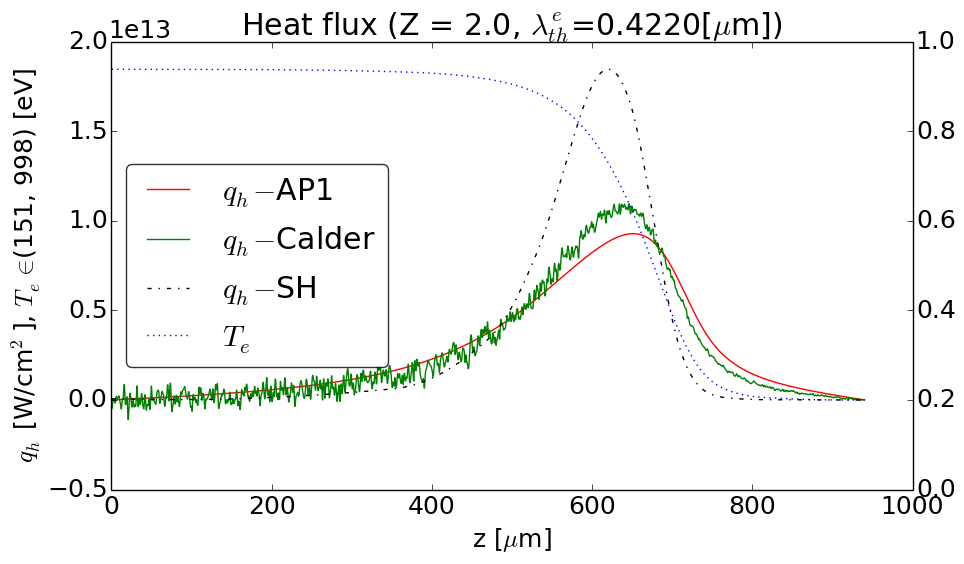
\includegraphics[width=\figscale\textwidth]{../VFPdata/C7_Calder_case1_heatflux.png} 
	  \\ 
	  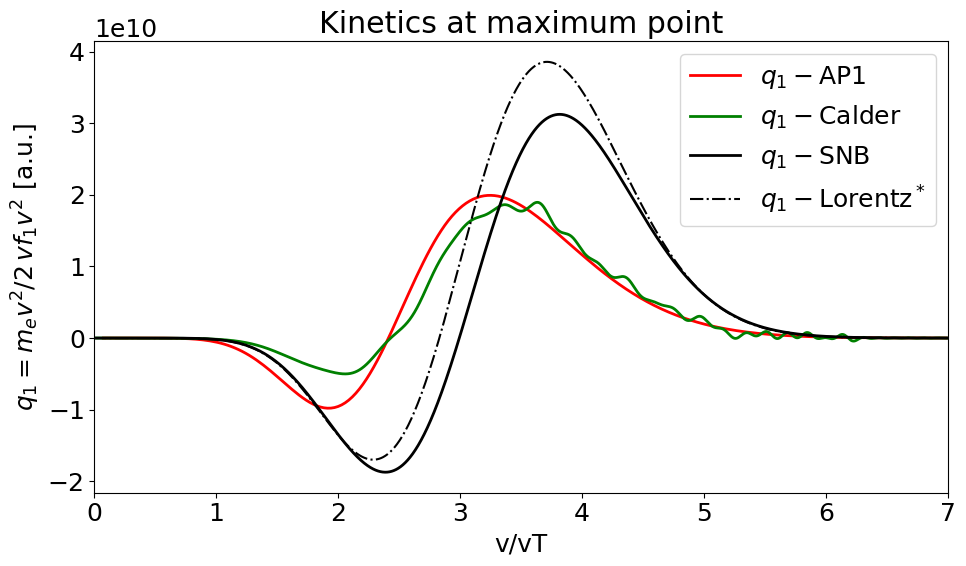
\includegraphics[width=\figscale\textwidth]{../VFPdata/C7_Calder_case1_kinetics.png}
	  \\ 
	  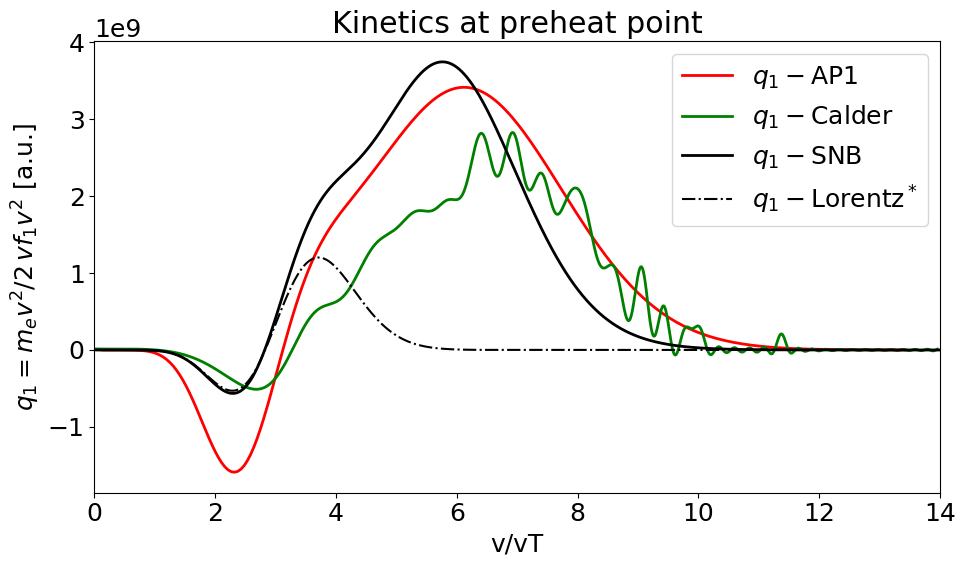
\includegraphics[width=\figscale\textwidth]{../VFPdata/C7_Calder_case1_nonlocal_kinetics.png}
    \end{tabular}
  \caption{  
  Snapshot 11 ps. Left: correct steady solution of heat flux. 
  %Right: AP1 kinetic profiles at point 750~$\mu$m corresponding to 
  %a~highly nonlocal nature of the~heat flux and is in a~good agreement with
  %\cite{Sherlock_PoP2017}. Velocity $max(q_1)$ = 5.8 $\vth$. 
  Velocity limit 6.4 $\vth$.
  }
  \label{fig:C7_Calder_case1}
  \end{center} 
\end{figure}

\subsection{Heat-bath problem}  
\label{sec:heatbath_test}

%\begin{figure}[tbh]
%  \begin{center}
%    \begin{tabular}{c}
%      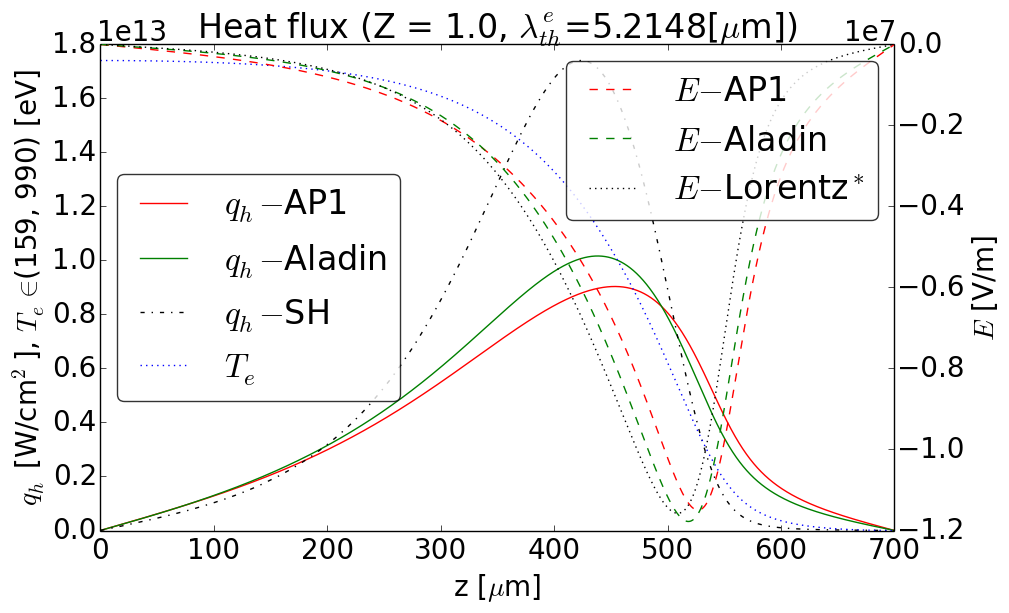
\includegraphics[width=\figscale\textwidth]{../VFPdata/C7_Aladin_case5_heatflux.png} \\
%      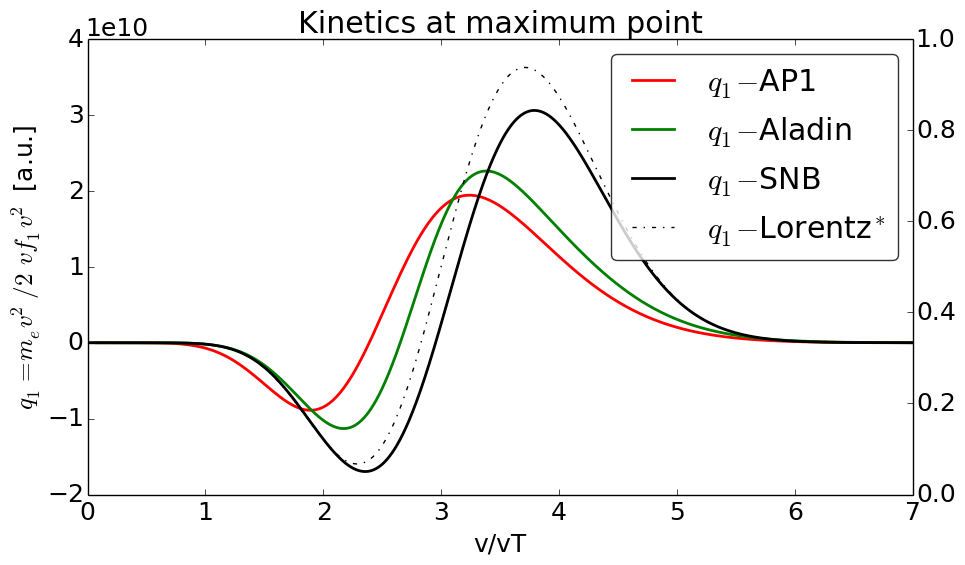
\includegraphics[width=\figscale\textwidth]{../VFPdata/C7_Aladin_case5_kinetics.png}
%    \end{tabular}
%  \caption{  
%  Snapshot 20 ps. Left: correct steady solution of heat flux. 
%  Right: Aladins results are correct. Velocity limit 4.4 $\vth$..
%  }
%  \label{fig:C7_Aladin_case5}
%  \end{center} 
%\end{figure}
\begin{figure}[tbh]
  \begin{center}
    \begin{tabular}{c}
      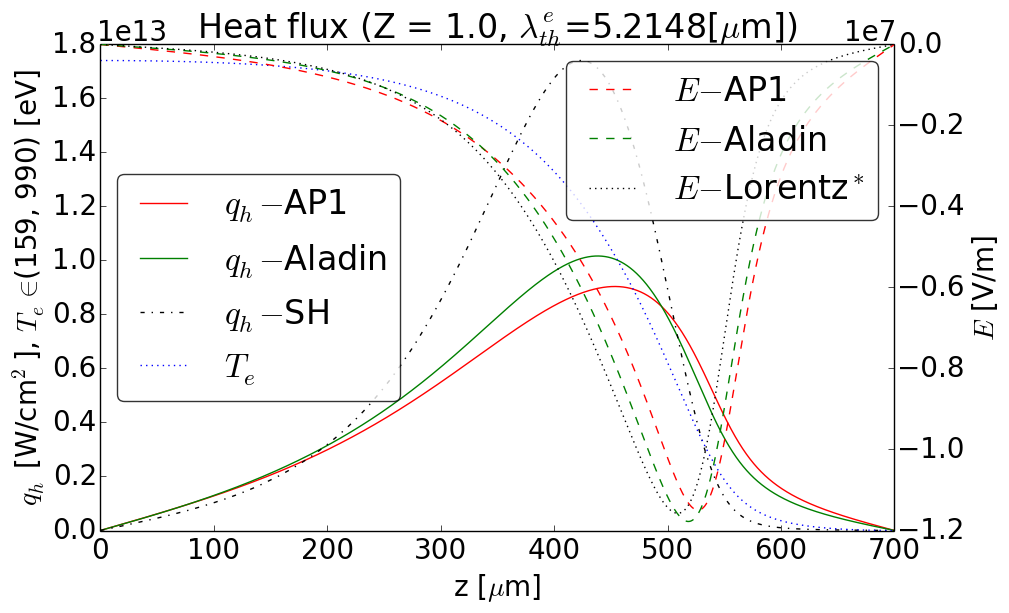
\includegraphics[width=\figscale\textwidth]{../VFPdata/C7_Aladin_case5_heatflux.png} \\
      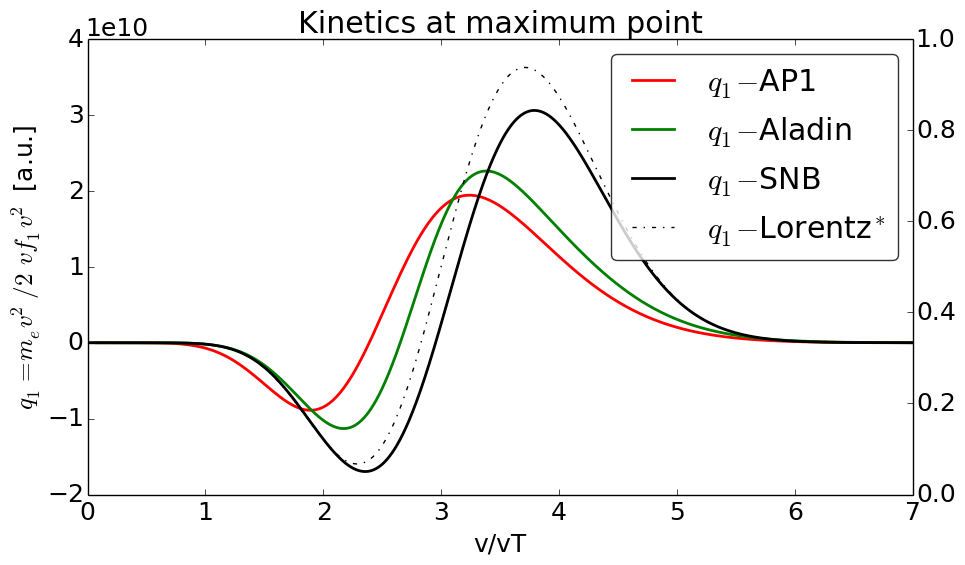
\includegraphics[width=\figscale\textwidth]{../VFPdata/C7_Aladin_case5_kinetics.png} \\
	  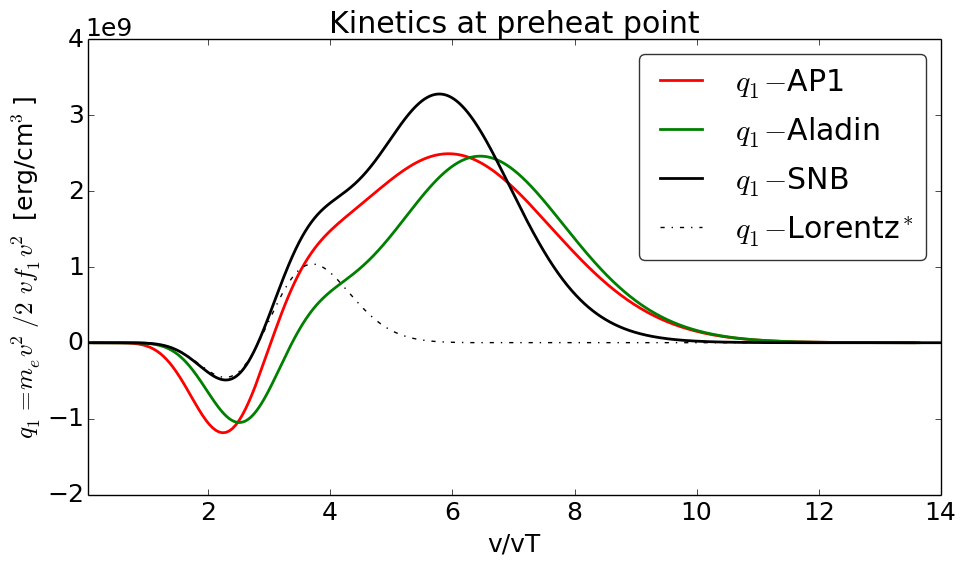
\includegraphics[width=\figscale\textwidth]{../VFPdata/C7_Aladin_case5_nonlocal_kinetics.png}
    \end{tabular}
  \caption{  
  Snapshot 20 ps. Top: correct steady solution of heat flux. 
  Right: Aladins results are correct. Velocity limit 4.4 $\vth$.
  Snapshot 20 ps. AP1 kinetic profiles at point 580~$\mu$m corresponding to 
  a~highly nonlocal nature of the~heat flux %\figref{fig:C7_Aladin_case5} 
  and is in a~good agreement with
  \cite{Sherlock_PoP2017}. Velocity $max(q_1)$ = 6.0 $\vth$. 
  Velocity limit 9.0 $\vth$.
  }
  \label{fig:C7_Aladin_case5}
  %\label{fig:C7_Aladin_case5_nonlocal}
  \end{center} 
\end{figure}

The accuracy of the AP1 implementation is compared to Aladin, Impact and Calder
codes by calculating the heat flow in the case
where a~large relative temperature variation
\begin{equation}
  T_e(z) = 0.575 - 0.425 \tanh\left((z-450) s\right) ,
  \label{eq:T_init}
\end{equation}
which exhibits a~smooth steep gradient at point 450~$\mu$m 
connecting a~hot bath ($T_e = 1$~keV) 
and cold bath ($T_e = 0.17$~keV) and $s$ is the~parameter of steepness. 
This test is referred to as a~simple non-linear heat-bath problem and
originally was introduced in \cite{marocchino2013} and further investigated
in  \cite{Sorbo_2015, Sorbo_2016, Sherlock_PoP2017, Brodrick_PoP2017}.

%Aladin and Impact simulations showed an evolution of the heat flow
%from the local (due to initialising as a Maxwellian) to the
%nonlocal, with a reduced peak, over an initial transient
%phase (over which the temperature ramp flattened somewhat). 
%The transient phase was considered over when the
%ratio of the VFP heat flow to the expected local heat
%flow stopped decreasing. After the transient phase this
%ratio begins to slowly increase as the thermal conduction flattens 
%the temperature ramp and the ratio of the scalelength to mfp increases 
%(i.e. the thermal transport slowly becomes more local). 

The~total computational box size is 700 $\mu$m in the~case
of Aladin and Impact and 1000 $\mu$m in the~case of Calder.
We performed Aladin, Impact, and Calder simulations showing an~evolution of
temperature starting from the~initial profile \eqref{eq:T_init}. 
Due to an~inexact initial distribution function (approximated by Maxwellian),
the~first phase of the~simulation exhibits a~transient behavior of the~heat
flux. After several ps the~distribution adjusts properly to its nonlocal nature
and the~actual heat flux profile can be compared. 
We then take the temperature profile from Aladin/Impact/Calder and used 
our AP1 implementation to calculate the heat flow
it would predict given this profile. In~particular, the~AP1 results 
corresponding to the~evolved temperature profile by Aladin can be found
in \figref{fig:C7_Aladin_case5} and \figref{fig:C7_Aladin_case3} for 
$\Zbar = 1$ and $\Zbar = 10$ respectively. The~AP1 results computed on
the~evolved temperature profile for $\Zbar = 2$ 
%by Impact are shown in \figref{fig:C7_Impact_case3} and 
by Calder can be found in \figref{fig:C7_Calder_case1}.

For all heat-bath simulations the electron density, Coulomb logarithm and 
ionisation were kept constant and uniform.
The~coulomb logarithm was held fixed throughout, 
$\lnc = 7.09$.
Nevertheless, the~Knudsen number Kn$^e$ has been varied among the~simulation 
runs in order to address a~broad range of nonlocality of 
the~electron transport corresponding 
to the~laser-heated plasma conditions, i.e. Kn$^e \in (0.0001, 1)$. 
The~variation of Kn$^e$ arises from the~variation
of the~uniform electron density $n_e \in (10^{19}, 10^{23})$ cm$^{-3}$ or 
the~length scale given by the~slope of the~temperature profile 
$s \in (1/2500, 1/25) \mu$m. Results of an~extensive set of simulations of
varying Kn$^e$ is shown in \figref{fig:Kn_results}.
 
\begin{figure}[tbh]
  \begin{center}
    \begin{tabular}{c}
      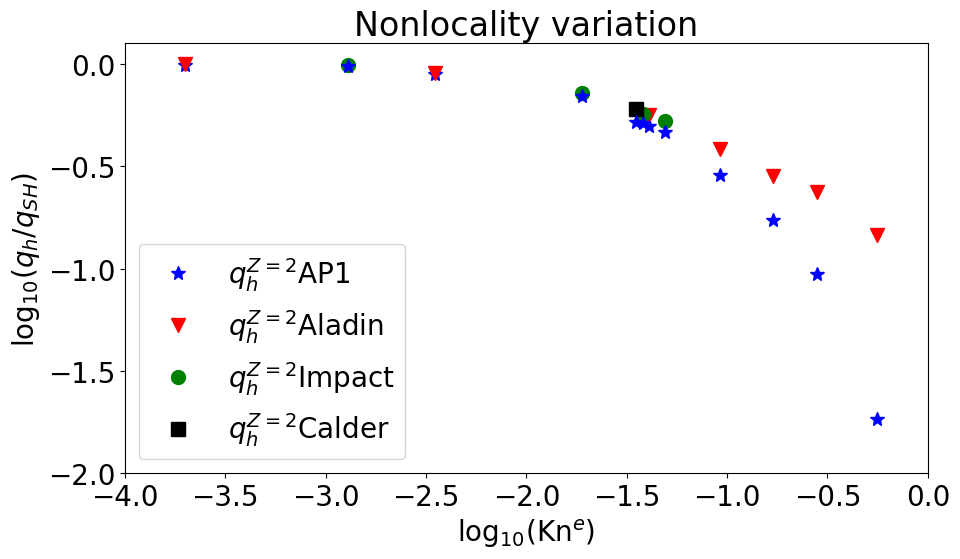
\includegraphics[width=\figscale\textwidth]{Kn_results.png}
    \end{tabular}
  \caption{  
  Simulation results for the case $Z=2$ computed by AP1/Aladin/Impact/Calder.
  Every point corresponds to the maximum heat flux in a "tanh" temperature 
  simulation, which can be characterized by Kn. The range of 
  $\log_{10}(\text{Kn})\in (0, -4)$ can be expressed as equivalent 
  to the~electron density approximate range n$_e \in (1e19, 3.5e22)$ of 
  the~50 $\mu$m slope tanh case. In the case of Kn = 0.56, 
  $q_{Aladin} / q_{AP1}\approx 7.9$.}
  \label{fig:Kn_results}
  \end{center} 
\end{figure}

Apart from the~distribution function details related to the~point of 
the~heat flux maximum, in \figref{fig:C7_Aladin_case5}
we also present the~detail of the~kinetic profile at point 580~$\mu$m 
corresponding to a~highly nonlocal nature of the~heat flux profile. 
Here a~good agreement with \cite{Sherlock_PoP2017} can be found.

When analyzing the~results of \figref{fig:Kn_results} we have found 
an~interesting observation related to stopping effect of electrons.
It turns out, that the~force acting on electrons is dominated by electric field
above some velocity limit $\vmag_{lim}$ and this limit drops down significantly
when the~plasma conditions are more nonlocal, i.e. with increasing Knudsen 
number as can be seen in \tabref{tab:vlim}.

\begin{table}
\begin{center}
  \begin{tabular}{c|ccccc}
    \hline\hline\\
    %Kn$^e$ & $10^{-4}$ & $10^{-3}$ & $10^{-2}$ & $10^{-1}$ & $1$ \\\\
    Kn$^e$ & $\,\,10^{-4}\,\,$ & $\,\,10^{-3}\,\,$ & $\,\,10^{-2}\,\,$ & $\,\,10^{-1}\,\,$ & $\,\,1\,\,$ \\\\
    \hline\\
    $\vmag_{lim} / \vth$ & 70.8 & 22.4 & 7.3 & 3.1 & 1.8\\\\
    \hline\hline
  \end{tabular}
  \caption{
  Scan over varying nonlocality (Kn$^e$) showing the~limit of 
  the~collision friction dominance over the~acceleration of electrons 
  due to the~electric field force. The~electric field effect is dominant
  for electrons with higher velocity than $\vmag_{lim}$ defined in 
  \eqref{eq:v_limit}. Kn$^e$ and $\vth$ are evaluated from the~same 
  plasma profiles.
  %$\sqrt{3}\vmag\frac{\me}{2\qe}\nue > |\E|$.
  }
\label{tab:vlim}
\end{center}
\end{table}

For practical reasons we present in \tabref{tab:vlim} 
some explicit values of velocity limit corresponding to varying transport 
conditions expressed in terms of "$\Zbar$" Knudsen number 
$\text{Kn}^e = \frac{\mfpe}{\sqrt{\Zbar + 1}L_{T_e}}$, 
where $\sqrt{\Zbar + 1}$ provides a~proper scaling of nonlocality with respect
to ionization, i.e. the~effect of scattering of electrons on ions 
\cite{LMV_1983_7}.

In every simulation run of AP1 we used 250~velocity groups in order to avoid
numerical errors in modeling of the~electron kinetics. However, a~smaller 
number of groups, e.g. 50, provides a~very similar results 
(an~error around 10$\%$ in the~heat flux).

\subsection{Hohlraum problem}
%While comparisons between the AP1 model and VFP
%codes have previously been performed 8,45 , none have included 
%spatially-inhomogeneous ionisation. 
Additionally to the~steep temperature gradients, the~laser-heated plasma 
experiments also involve steep density gradients and variation in ionization,
which is even more dominant in multi-material targets as in inertial
fusion experiments, e.g. at the interface between the helium gas-fill and 
the ablated high $\Zbar$ plasma.
%, it is critical that the AP1 model be tested 
%in such an environment.

In~\cite{Brodrick_PoP2017}, a~kinetic simulation of such a~test was introduced.
Plasma profiles provided by a~HYDRA simulation in 1D spherical
geometry of a~laser-heated gadolinium hohlraum containing a~typical helium 
gas-fill were used as input for the~IMPACT \cite{Kingham_JCP2004} VFP code. 
Electron temperature $T_e$, electron density $n_e$ and ionisation $\Zbar$ 
profiles shown in \figref{fig:Gd_VFP_10ps_heatflux} at 20 nanoseconds of 
the~HYDRA simulation were used (after spline smoothing) as 
the~initial conditions for the~IMPACT run (in planar geometry). 
For simplicity, the Coulomb logarithm was treated as a
constant $\lnc_{ei}$ = $\lnc_{ee}$ = 2.1484. In reality, in the~low-density 
corona $\lnc$ reaches 8, which, however, does not affect the~heat flux profile 
significantly. 
%Note that in reality
%5the plasma is only strongly coupled in the colder region of
%the gadolinium bubble beyond $\sim$1.7 mm and $\lnc_{ei}\approx$ 8
%up to $\sim$1.6 mm in the hotter corona.

It is worth mentioning that in the~surroundings of the~heat flux maximum 
($\sim 1662 \mu$m) the~profiles of all plasma variables exhibit steep gradients 
with a change from $T_e$ = 2.5 keV, $n_e$ = 5$\times$10$^{20}$ cm$^{−3}$, 
$\Zbar$ = 2 to $T_e$ = 0.3 keV, $n_e$ = 6$\times$10$^{21}$ cm$^{−3}$ , 
$\Zbar$ = 44 across approximately 100 $\mu$m 
(between 1600~$\mu$m and 1700~$\mu$m), starting at the~helium-gadolinium 
interface.  

%Reflective boundary
%conditions were used here as in the previous section and
%IMPACT used a timestep of 1.334 fs. The $n_e$ and $\Zbar$ profiles did not 
%evolve in the IMPACT simulation due to the treatment of the electric field 
%discussed in section II that ensures quasineutrality and the neglection of 
%ion motion and ionisation models.

%As with the VFP simulations in the previous section,
%there is an initial transient phase where the IMPACT
%heat flux gradually reduces from the Braginskii prediction
%as the distribution function rapidly moves away from
%Maxwellian. Once again this transient phase is considered
%to be over when the ratio of the peak heat flow to the
%Braginskii prediction stops reducing. This ratio is not
%observed to change by more than 5\% after the first 5 ps
%of our 15.7 ps simulation. Therefore, we conclude that
%it safe to assume the transient phase is over after 5 ps,
%at which point the temperature front has advanced by
%approximately 8 $\mu$m leading to a maximum temperature
%change of 41\% as shown in \figref{fig:Gd_VFP_10ps_heatflux}.

%In comparing the IMPACT, AP1, and SNB heat flow profiles
%we encountered an important subtlety concerning the implementation of 
%the model. A~recent SNB model with separate electron
%ion and electron-electron collision frequencies provides a
%very good prediction of the preheat into the hohlraum, the
%peak heat flow to within 16\% and an improved estimate
%of the thermal conduction in the gas-fill region, the latter
%is still too large by a factor of $\sim$2. This discrepancy could
%potentially lead to an overestimate of hohlraum temperatures and thus cause 
%issues similar to those arising with
%using an overly restrictive flux limiter.

\begin{figure}[tbh]
  \begin{center}
    \begin{tabular}{c}
      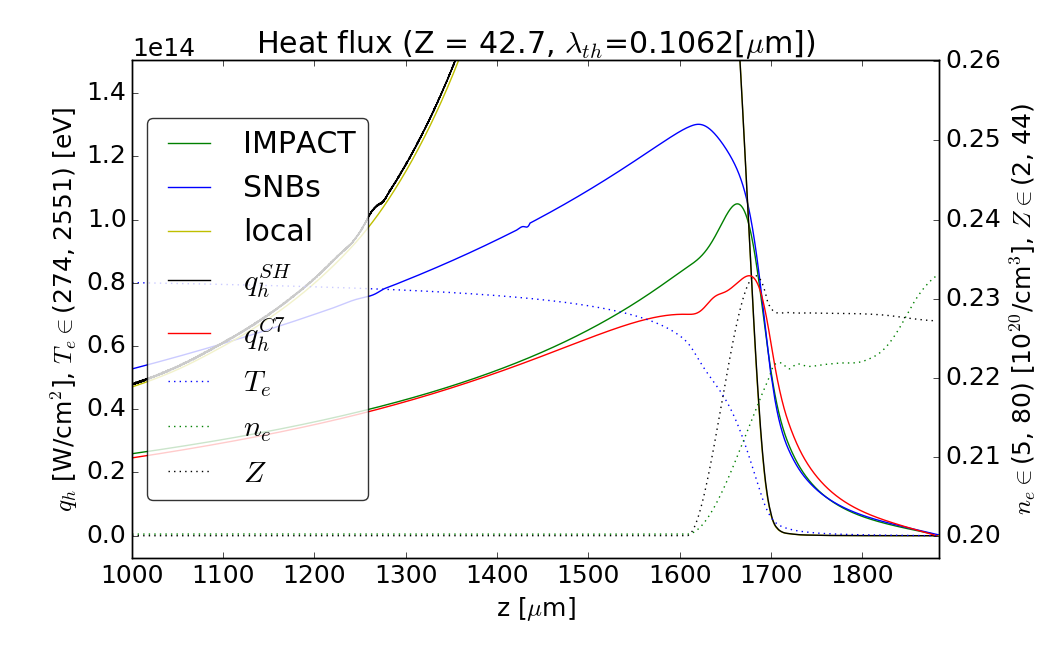
\includegraphics[width=\figscale\textwidth]{../VFPdata/GD_Hohlraum/fluxes_10ps.png} 
    \end{tabular}
  \caption{
  }
  \label{fig:Gd_VFP_10ps_heatflux}
  \end{center} 
\end{figure}

%\begin{itemize}
%  \item Multiple runs analyzing the~performance of AP1 with respect to 
%    Aladin/Impact/Calder along wide range of Kn$^e$ shown in 
%    \figref{fig:Kn_results}.
%  \item Realistic hydro simulation setting provided by HYDRA, a~comparison
%    between AP1, Impact, and SNB shown in \figref{fig:Gd_VFP_10ps_heatflux}.
%  \item Comment on and summarize the~velocity limits for all figs.
%\end{itemize}

%
